\subsection{Model}
\label{sub:modelComponent}
The class diagram showed in figure \ref{fig:pdaclassdiagram} is altered to apply the MVC design pattern.
The new class diagram can be seen on figure \ref{fig:ClassDiagramV2}.
Each class will be described in detail in the following.
\begin{figure}[p]%
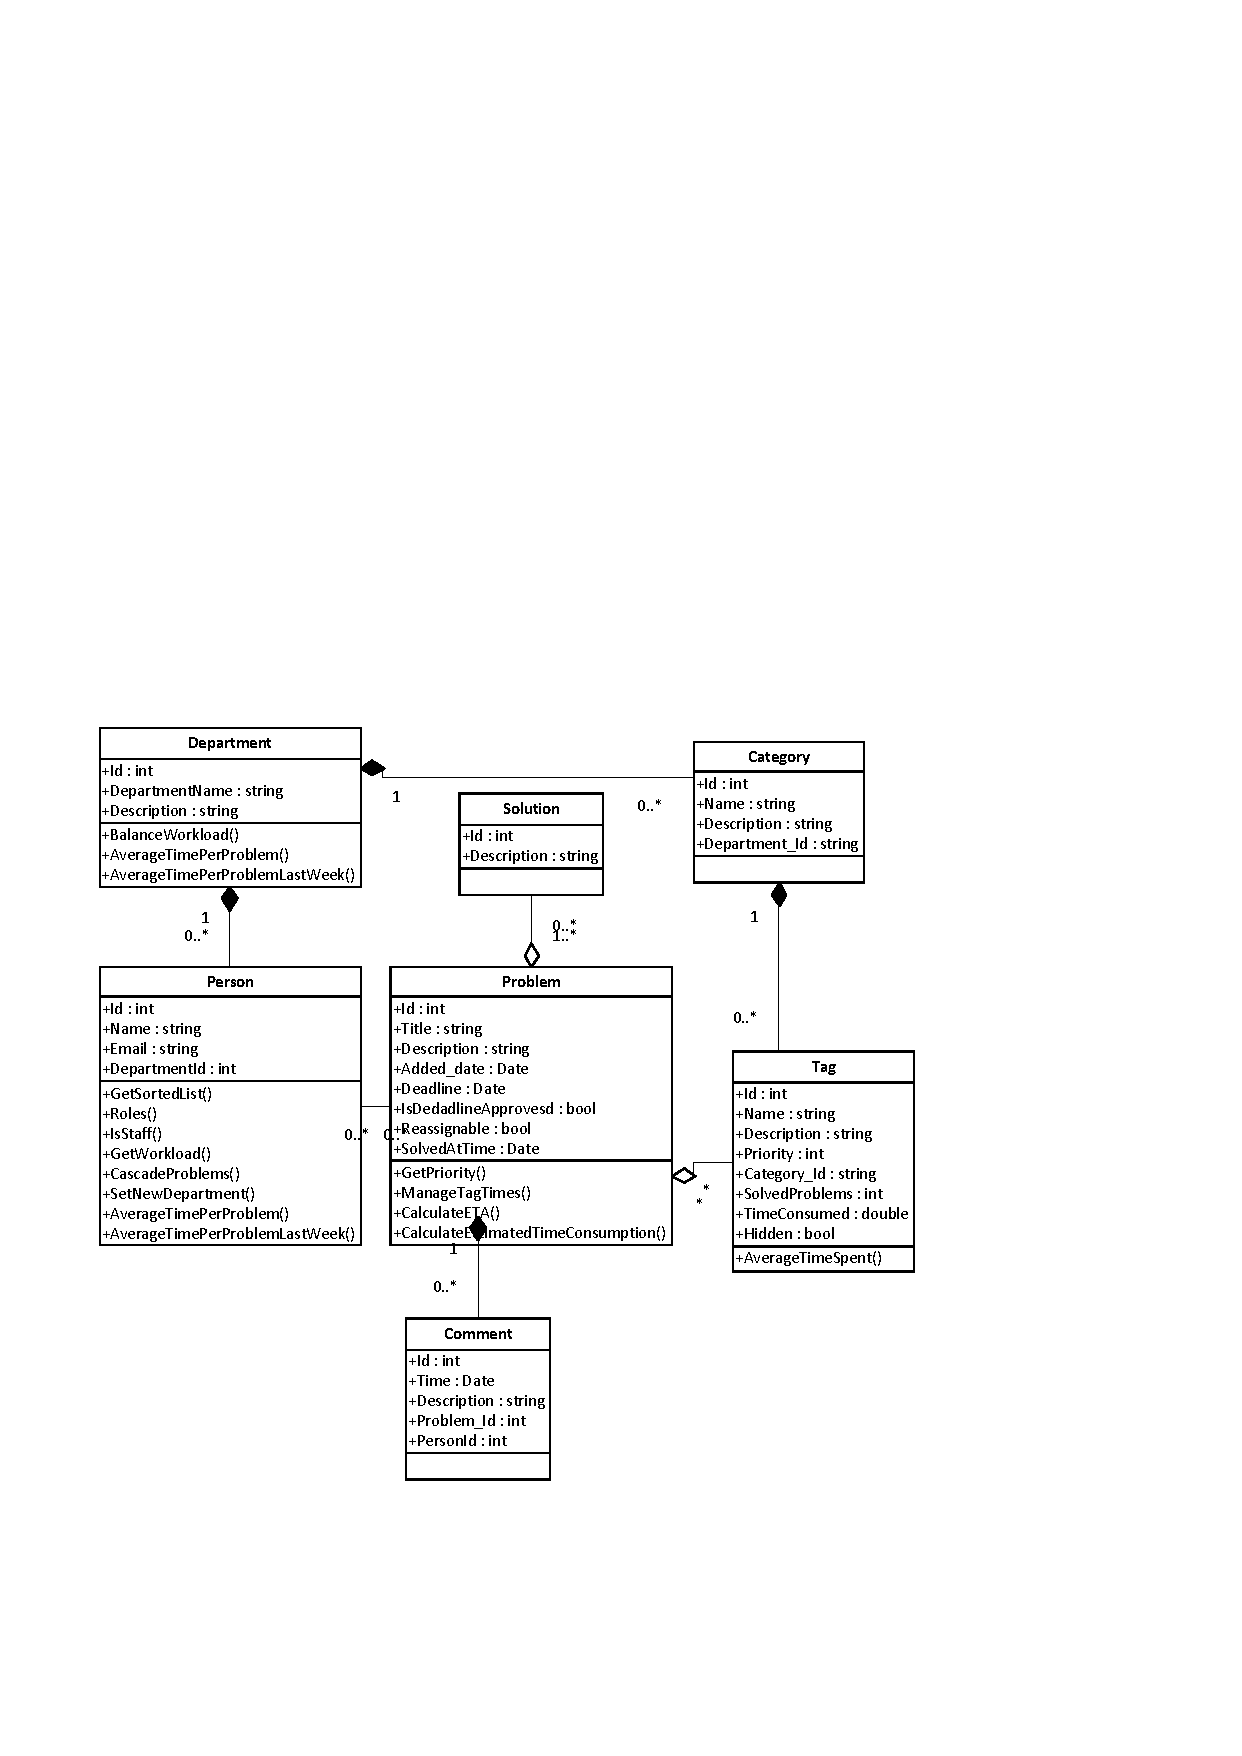
\includegraphics[clip=true, width=1.00\textwidth, trim=0.5cm 5cm 7.5cm 7cm]{input/component_design/ClassDiagramV2.pdf}%
\morscaption{The class diagram}%
\label{fig:ClassDiagramV2}%
\end{figure}

%The altered version of our class diagram contains the following changes:
%\begin{itemize}	
%	\item The role pattern: \\
%	The functionality from the actor \admin[] does not inherit from \astaff[] and \aclient[] etc. Figure \ref{tab:newactortable} shows the new role system.   
%	\item Problem: 
%	\begin{itemize}
%		\item \textbf{Deadline} \\
%					The deadline is now a attribute instead of a class
%		\item \textbf{Problem and tag relation} \\
%					A tag can be connected to multiple different problems and a problem can have many tags connected to it. 
%		\item \textbf{Problem and person relations} \\
%					A person can have from zero to three simultaneous roles.				
%	\end{itemize}
%\end{itemize} 




%%\subsubsection{Description of Attributes for Each Class}
There are additional navigation properties on some of the classes such as the \vari{Solutions} attribute on \cl{Problem}, which lists the attached solutions.
These are not outlined below as they are generated by the ADO.NET entity frame.
ADO.NET is described in section \ref{sub:adonet}.
\begin{description}
\item[Problem]\hfill
\begin{description}
	\item[Purpose:]To represent problems and their relations to persons, comments, tags, and solutions.
	\item[Attributes:]Id, Title, Description, Added\_date, Deadline, IsDeadlineApproved, Reassignable, and SolvedAtTime
	\item[Operations:]\me{GetPriority} -- the priority of the problem, \me{MangeTagTimes} -- saves the solve time to the tags attached to the problem, \me{CalculateETA} -- calculates the estimated time of completion, and  \me{CalculateEstimatedTimeConsumption} -- calculates the estimated time consumption.
%\item[Id:] A unique number which identifies each problem. 
%\item[Title:] Contains the problems title.
%\item[Description:] Contains the problems description.
%\item[Added\_date:] The date and time of when the problem is added.
%\item[Deadline:] A field where a date with a deadline can be added.
%\item[IsDeadlineApproved:] Whether or not the problems deadline has been approved by the assigned \astaff[] member.
%\item[Reassignable:] Whether or not a problem can be reassigned by the balance workload function \ref{sec:balanceworkload}. 
%\item[SolvedAtTime:] If a problem has been solved, the time of completion is saved, if there is no SolvedAtTime then the problems status is unsolved.
\end{description}
\end{description}

\begin{description}
\item[Person]\hfill
\begin{description}
	\item[Purpose:]To represent the persons using our application and their relations, as well as perform operations associated with a person.
	\item[Attributes:]Id, Name, Email, and DepartmentId
	\item[Operations:]\me{GetSortedList} -- gets the worklist for a \astaff[] member in sorted order, \me{Roles}, \me{IsStaff}, \me{GetWorkload}, \me{CascadeProblems} -- reassign the problems to other \astaff[] members of a given department, \me{SetNewDepartment}, \me{AverageTimePerProblem} -- gives the average time it takes for problems to be solved, and \me{AverageTimePerProblemLastWeek} -- gives the average time it takes for problems to be solved during the last seven days.
%\item[Id:] A number which is unique for each Person. 
%\item[Name:] The name of the person.
%\item[Email:] The persons email, notifications are send to this email.  
%\item[DepartmentId:] This the id of the persons department if any. 
\end{description}
\end{description}

\begin{description}
\item[Department]\hfill
\begin{description}
	\item[Purpose:]To represent departments and their relations, as well as handle some statistics and balance the workload across the persons associated with the department.
	\item[Attributes:]Id, DepartmentName, and Description
	\item[Operations:]\me{BalanceWorklaod} -- balances the problems between \astaff[] members of the department, \me{AverageTimePerProblem} -- gives the average time it takes for problems to be solved, and \me{AverageTimePerProblemLastWeek} -- gives the average time it takes for problems to be solved during the last seven days.
%\item[Id:] A number which is unique for each department. 
%\item[DepartmentName:] The name of the department.
%\item[Description:] Contains the description of the department.
\end{description}
\end{description}

\begin{description}
\item[Solution]\hfill
\begin{description}
	\item[Purpose:]To represent solutions and their relations.
	\item[Attributes:]Id and Description
	\item[Operations:]none
%\item[Id:] A number which is unique for each solution. 
%\item[Description:] Contains the solution.
\end{description}
\end{description}

\begin{description}
\item[Category]\hfill
\begin{description}
	\item[Purpose:]To represent categories and their relations to departments and tags.
	\item[Attributes:]Id, Name, Description, and Department\_Id
	\item[Operations:]none
%\item[Id:] A number which is unique for each category. 
%\item[Name:] The name of the category.
%\item[Description:] Contains the description of the category.
%\item[Department\_Id:] The id of the department which the category belongs to. 
\end{description}
\end{description}

\begin{description}
\item[Tag]\hfill
\begin{description}
	\item[Purpose:]To represent tags and their relations to categories and problems. 
	\item[Attributes:]Id, Name, Description, Priority, Category\_Id, SolvedProblems, TimeConsumed, and Hidden
	\item[Operations:]\me{AverageTimeSpent} -- the average time to solve problems with the given tag.
%\item[Id:] A number which is unique for each tag. 
%\item[Name:] The name of the tag.
%\item[Description:] The description of the tag.
%\item[Priority:] Each tag have a weight, problems with high weight are prioritized higher.
%\item[Category\_Id:] The id of the category which the tag belongs to. 
%\item[SolvedProblems:] The number of problems which have been solved with this tag.
%\item[TimeConsumed:] The total time problems with this tag have required to solve.
%\item[Hidden:] Whether or not a tag is visible.
\end{description}
\end{description}

\begin{description}
\item[Comment]\hfill
\begin{description}
	\item[Purpose:]To represent comments and their relations to persons and problems.
	\item[Attributes:]Id, Time, Description, Problem\_Id, and PersonId
	\item[Operations:]none
%\item[Id:] A number which is unique for each comment. 
%\item[Time:] The time and date when the comment is posted.  
%\item[Description:] The content of the comment.
%\item[Problem\_Id:] The id of the problem which the comment belongs to.
%\item[PersonId:] The id of the person who wrote the comment.
\end{description}
\end{description}
